\documentclass[a4paper,10pt,review]{elsarticle}

\usepackage{lineno,hyperref} % Use this line to activate reference hyperlinks
% \usepackage{lineno} % Use this line to deactivate reference hyperlinks for ease of reviewing
\modulolinenumbers[5]

% START: Inserted by AJS
\frenchspacing
\usepackage{ifxetex}
\ifxetex
  \usepackage{fontspec}
  \defaultfontfeatures{Ligatures=TeX} % To support LaTeX quoting style
  \setromanfont{Hoefler Text}
  % \setmainfont[Ligatures=TeX]{Palatino}
\else
  \usepackage[T1]{fontenc}
  \usepackage[utf8]{inputenc}
  \usepackage{lmodern}
  \usepackage{textcomp} % directly use the degree (and some other) symbol
\fi

% \usepackage{fixltx2e}
\usepackage[]{graphicx}
\usepackage{wrapfig}
\usepackage{lscape}
\usepackage{rotating}
\usepackage{epstopdf}
\usepackage{ragged2e}  % for '\RaggedRight' macro (allows hyphenation)
\usepackage[pdftex]{color}
\usepackage[margin=2.75cm]{geometry}
\usepackage{upquote}
\usepackage{textgreek}
\usepackage{microtype} % place after fonts; even better typesetting for improved readability
\usepackage{xfrac} % nice fractions
\usepackage{booktabs} % nice tables without vertical lines
\setlength\heavyrulewidth{0.1em}
\setlength\lightrulewidth{0.0625em}
\usepackage[color=yellow, textsize=tiny]{todonotes}
\usepackage[font={small}, labelfont=bf]{caption} % tweaking the captions
\usepackage{gensymb}
\usepackage{amsmath,amssymb}
\usepackage{cleveref} % clever cross referencing figures and tables; last package to include
% END: Inserted by AJS
\usepackage{natbib}

\journal{Progress in Oceanography}

%%%%%%%%%%%%%%%%%%%%%%%
%% Elsevier bibliography styles
%%%%%%%%%%%%%%%%%%%%%%%
%% To change the style, put a % in front of the second line of the current style and
%% remove the % from the second line of the style you would like to use.
%%%%%%%%%%%%%%%%%%%%%%%

%% Numbered
%\bibliographystyle{model1-num-names}

%% Numbered without titles
% \bibliographystyle{model1a-num-names}

%% Harvard
% \bibliographystyle{model2-names.bst}\biboptions{authoryear}

%% Vancouver numbered
%\usepackage{numcompress}\bibliographystyle{model3-num-names}

%% Vancouver name/year
% \usepackage{numcompress}\bibliographystyle{model4-names}\biboptions{authoryear}

%% APA style
% \bibliographystyle{model5-names}\biboptions{authoryear}

%% AMA style
%\usepackage{numcompress}\bibliographystyle{model6-num-names}

%% `Elsevier LaTeX' style
% \bibliographystyle{elsarticle-num}
\bibliographystyle{elsarticle-harv}\biboptions{authoryear}
% \bibliographystyle{elsarticle-num-names}
%%%%%%%%%%%%%%%%%%%%%%%

\begin{document}

\begin{frontmatter}

\title{Predominant air-sea patterns during coastal marine heatwaves}

%% or include affiliations in footnotes:
\author[firstaddress]{Robert W. Schlegel\corref{mycorrespondingauthor}}
\cortext[mycorrespondingauthor]{Corresponding author}
\ead{3503570@myuwc.ac.za}
\author[secondaddress,thirdaddress,fourthaddress]{Eric C. J. Oliver}
\author[fifthaddress]{Sarah Perkins-Kirkpatrick}
\author[sixthaddress,seventhaddress]{Andries Kruger}
\author[firstaddress]{Albertus J. Smit}
% \author[mysecondaryaddress]{Global Customer Service\corref{mycorrespondingauthor}}

\address[firstaddress]{Department of Biodiversity and Conservation Biology, University of the Western Cape, Private Bag X17, Bellville 7535, South Africa}

\address[secondaddress]{Australian Research Council Centre of Excellence for Climate System Science, Australia}

\address[thirdaddress]{Institute for Marine and Antarctic Studies, University of Tasmania, Hobart, Australia}

\address[fourthaddress]{Department of Oceanography, Dalhousie University, Halifax, Nova Scotia, Canada}

\address[fifthaddress]{UWA Oceans Institute and School of Plant Biology, The University of Western Australia, Crawley, 6009 Western Australia, Australia}

\address[sixthaddress]{Climate Service, South African Weather Service, Pretoria, South Africa}

\address[seventhaddress]{Department of Geography, Geoinformatics and Meteorology, Faculty of Natural and Agricultural Sciences, University of Pretoria, South Africa}


\begin{abstract}
As the mean temperatures of the worlds oceans increase, it is predicted that marine heatwaves (MHWs) will occur more frequently and with increased severity however, it has been shown that a range of variables have been responsible for these extreme events. An improved understanding of the mechanisms driving MHWs at specific localities may allow us to better forecast their occurrence. To this end we have utilized atmospheric (ERA-Interim) and oceanic (OISST, AVISO) data to examine the air-sea states around southern Africa during coastal (<400 m from the low water mark; measured \emph{in situ}) MHWs. Nonmetirc multidimensional scaling (NMDS) was first used to determine that MHW states were different from daily climatological states. Self-organising maps (SOMs) were then used to cluster the MHW states into one of nine nodes to determine the predominant air-sea patterns present during these events. It was found that warm water forced onto the coast via anomalous ocean circulation was the predominant oceanographic pattern during most MHWs. A range of distinct air temperature and wind patterns were found with warm air temperatures over the subcontinent during onshore or alongshore winds featuring most prominently during MHWs. It may therefore be possible to forecast the occurrence of MHWs when such air and sea states are projected to occur simultaneously. The lack of any strong air-sea patterns during roughly one third of the MHWs implied that they were not forced by a recurring air-sea state, but rather through the unpredictable chaos of the climate system.
% The lack of any strong air-sea patterns during roughly one third of the MHWs implied that sub-meso-scale activity may have been responsible for them and that finer scale observations may be necessary to deduce their physical drivers. 
% These findings motivate for the implementation of local scale real-time \emph{in situ} monitoring of at risk coastal locations in conjunction with the development of a forecasting and disaster prevention system.
\end{abstract}

\begin{keyword}
marine heatwaves \sep extreme events \sep coastal \sep atmosphere \sep ocean \sep reanalysis data \sep \emph{in situ} data \sep climate change
\end{keyword}

\end{frontmatter}

\linenumbers

\section{Introduction}
The anthropogenically forced warming of air, land, and sea have been widely publicized over the last several decades \citep[e.g.][]{Manabe1967, Sawyer1972, Hansen1981, Cox2000, Rosenzweig2008}. Investigations into the negative impacts this warming may have on ecosystems range in focus from long term trends \citep[e.g.][]{Scavia2002, Walther2002, Burrows2011} to shifting states \citep[e.g.][]{Travis2003, Grebmeier2006, Blamey2015} to extreme individual events \citep[e.g.][]{Easterling2000, Barrett2008, Wernberg2012a}. Whereas long term temperature trends are projected to have a negative impact on many of Earth's systems \citep{IPCC2014}, and the shifts in thermal states brought about by these long term trends are projected to cause irreversible species loss \citep{Thomas2004}, extreme events pose a more immediate threat to ecosystems \citep[e.g.][]{Jolly2005, Denny2009, Hufkens2012}. Extreme thermal events have been given a range of labels but are broadly divided into two categories: cold-spells \citep[e.g.][]{Gunter1941, Lirman2011, Boucek2016} and heatwaves \citep[e.g.][]{Gordon1988, Stott2004, Perkins-Kirkpatrick2016}. We chose here to focus on heatwaves that occur in the sea, classified as 'marine heatwaves' (MHWs) \citep{Hobday2016}.

Several large MHWs, and their ecological impacts, have been well documented. The first is a 2003 MHW that negatively impacted as much as 80\% of the Gorgonian fan colonies in the Mediterranean \citep{Garrabou2009}. A 2011 MHW is now known to have caused a permanent ~100 km range contraction of the ecosystem forming-kelp species \emph{Ecklonia radiata} in favour of the tropicalisation of reef fishes and seaweed turfs along the southern coast of Western Australia \citep{Wernberg2016}. The damage caused by MHWs is not confined to demersal organisms or coastal ecosystems as demonstrated by a MHW in the North West Atlantic Ocean in 2012 that impacted multiple commercial fisheries \citep{Mills2013}. When extreme enough, such as ``the Blob'' that persisted in the North West Pacific Ocean from 2014 to 2016, a MHW may negatively impact even marine mammals and seabirds \citep{Cavole2016}. Besides increases in mortality due to thermal stress, MHWs may also lead to outbreaks of disease in commercially viable species, such as that which occurred during the 2015/16 Tasman Sea event \citep{Oliver2017}.
% Analyses of \emph{in situ} coastal seawater temperature time series from South Africa have shown that MHWs of comparable magnitude to those highlighted here have occurred \citep{Schlegel2017} however, it is not known what damage these events may have caused as little long-term ecological sampling is carried out where these events occurred.

It is now possible to directly compare MHWs occurring anywhere on the globe during any time of year using a consistent definition developed by \citet{Hobday2016}, which was accompanied by the development of a statistical methodology for calculating these events. Whereas the metrics created for the measurement of MHWs allowed for the comparison of events, they did not directly reveal what may be causing them. Beyond common measurements, it is necessary to identify the possible physical drivers of MHWs so as to be able to compare similar `types' of events and to be able to move towards a system of prediction.

It has been assumed that coastal MHWs should either be caused by oceanic forcing, atmospheric forcing, or a combination of the two; however, the scale at which this forcing must occur in order to drive MHWs at the coast has yet to be determined. Recent research into the rates of co-occurrence between nearshore and offshore MHWs revealed that oceanic forcing from offshore (within the continental shelf) onto the nearshore (<400 m from the coast, \emph{i.e.} also referred to as local scale) was far less responsible for the formation of coastal MHWs than hypothesised \citep{Schlegel2017}. It is therefore necessary to consider broader meso-scale mechanisms that may be responsible for such events occurring at the local scale. For example, the 2011 Western Australia MHW \citep{Pearce2013} was caused by the aseasonal transport of warm water onto the coast due to a surge of the Leeuwin Current \citep{Feng2013, Benthuysen2014}. Oceanic forcing was also the main contributor of the anomalously warm water during the 2015/16 Tasman MHW when the southward flowing East Australian Current caused a convergence of heat there \citep{Oliver2017}. Conversely, \citet{Garrabou2009} were able to show that atmospheric forcing played a clear role in formation of the 2003 Mediterranean MHW. While more complex, \citet{Chen2015a} also showed that air-sea heat flux could be attributed as the main forcing variable in the 2012 Atlantic MHW. ``The Blob'' however appears to have occurred due to the lack of advection of heat from surface waters into the atmosphere due to anomalously high sea level pressure \citep{Bond2015a}. Outside of these few examples for these well documented events there has been little progress in developing a global understanding of the forcing of MHWs.

In order to develop a methodology that could be used to investigate the potential air and/or sea forcing of multiple coastal MHWs within a single framework, an index of the mean synoptic air-sea states around southern Africa during the occurrence of these events was created, similar to \citet{Oliver2017atlas} for Eastern Tasmania. These states were then clustered with the use of a self-organising map (SOM). The aim of the clustering was to visualise synoptic and/or meso-scale patterns in the air and/or sea that occur during MHWs at coastal sites. We predicted that i) air-sea states during MHWs days would differ from the daily climatologies; ii) typical groupings of air and sea patterns would be revealed through clustering; iii) clustered oceanic patterns would occur in closer proximity to the coastal MHWs than the clustered atmospheric patterns; and iii) the air-sea states would aid in the development of a broader mechanistic understanding of the physical drivers of coastal MHWs.

\section{Material and Methods}
\subsection{Study region}
The \emph{ca}. 3,100 km long South African coastline provides a natural laboratory for investigations into the forcing of nearshore phenomena as it may be divided into three distinct sections, allowing for a range of meso-scale oceanographic influences to be considered within the same research framework (\Cref{figure1}) therefore, the extent of the study area was set at 10\degree E to 40\degree E and 25\degree S to 40\degree S. The range of temperatures experienced along all three coasts is large, and the gradient of increasing temperature from the border of Namibia (Site 1) to the border of Mozambique (Site 26) is nearly linear. The west coast of the country is distinct from the other two coasts as it is bordered by the Benguela Current, which forms an Eastern Boundary Upwelling System (EBUS) \citep{Hutchings2009} against the coast. Conversely, the east coast is dominated by a western boundary current, the Agulhas Current \citep{Luning1990}, a poleward flowing body of warm water. The south coast is also bordered by the Agulhas current but differs from the east coast in that it experiences both shear-forced and wind-driven upwelling \citep{Lutjeharms2000a} in addition to having significantly more thermal variability than present along  the other two coasts \citep{Schlegel2017}. The Agulhas and Benguela currents `battle' each other for a position of supremacy along the south coast of the subcontinent and no fixed border between the two exists. The meso-scale dance of these two mighty currents range from the Cape Peninsula in the west, to the western portion of the Agulhas Bank in the east. The Agulhas current  retroflects to the south, and then back to the east, upon coming into contact with the Benguela \citep{Hutchings2009} however, it will occasionally punch through into the South Atlantic. This event, known as Agulhas leakage, allows warm, saline eddies of Indian Ocean water to propagate into the Atlantic Ocean \citep{Beal2011}.

Atmospheric circulation over the study area is dominated by two quasi-stationary anticyclonic high pressure cells. The South Indian Ocean High (hereafter Indian high) is situated approximately on the eastern border of the study area and draws warm moist air towards the east coast, whereas the South Atlantic Ocean High (hereafter Atlantic high) is found to the west of the subcontinent and draws cool dry air onto the west coast \citep{vanHeerden1998}. To the south of the subcontinent, prevailing westerly winds blow south of these two high pressure cells \citep{vanHeerden1998}. From the mean wind pattern, these three atmospheric features can be discerned from \Cref{figure1}. Summer heating may lead to the development of heat lows within the subcontinent, which tend to be absent during winter \citep{Tyson2000}, allowing for the Indian and Atlantic highs to link over land \citep{vanHeerden1998}. Additionally, the Indian and Atlantic highs, as well as the westerlies, move northwards during winter months, with the effect that the colder westerly winds influence the weather mostly along the southern parts of the sub-continent \citep{vanHeerden1998}. Air temperatures along the coasts are largely influenced by the cold Benguela on the west coast and warm Agulhas current along the east and south coasts \citep{vanHeerden1998}.
% These synoptic patterns may be the driving force of wind movement over the subcontinet however, there are meso-scale features, particularly along the coast, that also affect wind movement and air temperature.

\begin{figure}
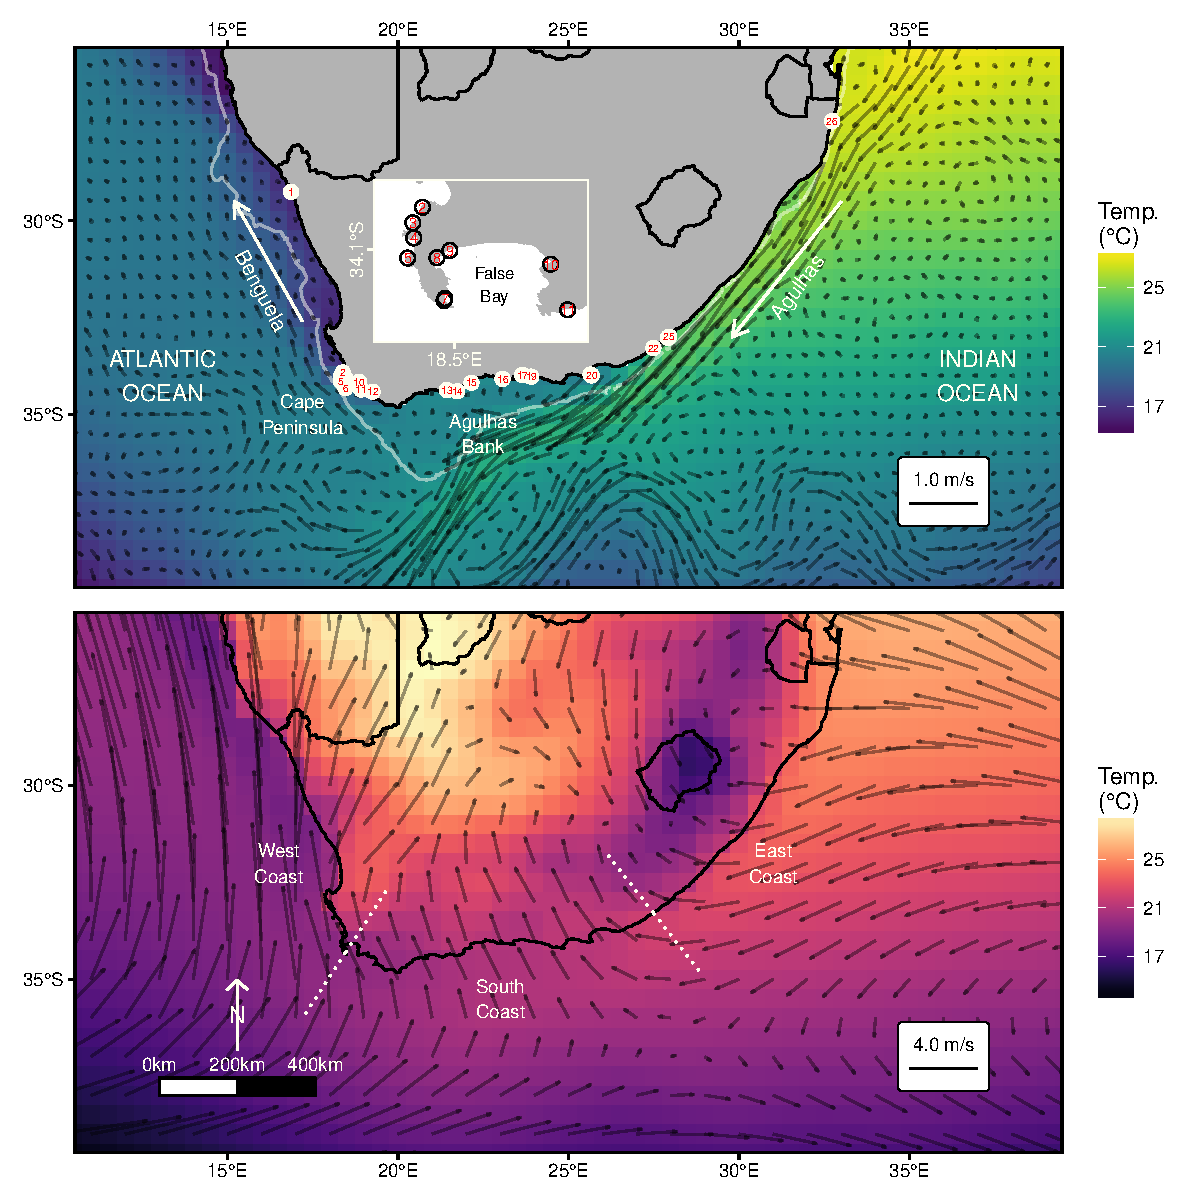
\includegraphics[width=1.0\textwidth]{figure_1.pdf}
\caption{Map of the study area where the top panel shows the mean annual sea surface temperature (SST) and surface currents from 1993 to 2016, as well as the locations referred to in the text. The sites of \emph{in situ} collection are shown with red numerals over white circles. An inset map of the Cape Peninsula/False Bay area is shown where site labels are obscured due to overplotting. The bottom panel shows the mean surface air temperature and winds, and highlights the three coastal sections found within the study area as well as the three predominant wind patterns. Note that the temperature and vector scales differ between the two panels. The white vector arrows showing the predominant ocean and atmosphere circulation patterns are approximations and not exact values.}
\label{figure1}
\end{figure}

\subsection{Data}
\subsubsection{\emph{In situ} data}
The \emph{in situ} coastal seawater temperature data used in this study were acquired from the South African Coastal Temperature Network (SACTN, https://github.com/ajsmit/SACTN, https://robert-schlegel.shinyapps.io/SACTN/). These data are contributed by seven different organizations and are collected \emph{in situ} with a mixture of hand-held alcohol or mercury thermometers as well as digital underwater temperature recorders (UTRs). This data set currently consists of 135 daily time series, with a mean duration of 19.7 years, meaning that many the time series in this dataset are shorter than the 30 year minimum proscribed for the characterisation of MHWs (see 'Marine heatwaves' section below) \citep{Hobday2016}. It is however deemed necessary to use these data when investigating extreme events in the nearshore (<400 m from the low tide mark) as satellite derived sea surface temperature (SST) values along the coast have been shown to display large biases \citep{Smit2013} or capture minimum and maximum temperatures poorly \citep{Smale2009, Castillo2010}. Whereas a 30+ year period is ideal for determining a climatology, ten years may serve as an acceptable bottom limit \citep{Schlegel2017}. Following on from the methodology laid out in \citet{Schlegel2017}, time series with more than 10\% missing data or shorter than 10 years in length were excluded from this research. Accounting for these 10 year length and 10\% missing data constraints, the total number of \emph{in situ} time series used in this study was reduced to 26, with a mean length of 22.3 years.

\subsubsection{Reanalysis data}
To visualise a synoptic view of the atmospheric state around southern Africa during coastal MHWs (see sections 'Marine heatwaves' and 'Air-sea state' below) we chose to use ERA-Interim to provide air temperatures (2 m above surface) and wind vectors (10 m above surface). ERA-Interim is a comprehensive global atmospheric model that assimilates a wide range of data to create short term forecasts for 60 vertical layers \citep{Dee2011}. These forecasts are then combined with the assimilated data again during each 12-hourly cycle \citep{Dee2011}. ERA-Interim is produced by the European Centre for Medium-Range Weather Forecasts (ECMWF, http://www.ecmwf.int/) and at the time of this writing the chosen variables were available for download from January 1st, 1979 to December 31st, 2016. The data used in this study were downloaded at a daily resolution on a 1/2\degree \: grid and within the latitude/longitude of the study region (\Cref{figure1}).

Research on oceanic reanalysis data around southern Africa have shown that none of the products currently available model the complex Agulhas current well \citep{Cooper2014}. It was therefore decided to use remotely sensed data to determine the sea surface temperature (SST) and surface currents in the study area.

\subsubsection{Remotely sensed data}
SST within the study region was determined with the AVHRR-Only Optimum Interpolated Sea Surface Temperature (OISST) dataset produced by NOAA. NOAA OISST is a global 1/4\degree \: gridded daily SST product that assimilates both remotely sensed and \emph{in situ} sources of data to create a level-4 gap free product \citep{Banzon2016}. These data were averaged to a 1/2\degree \: grid to match the courser resolution of the ERA-Interim data. At the time of this writing these data were available for download from September 1st, 1981 to June 5th, 2017.

To determine ocean surface currents remotely on a daily global 1/4\degree \: grid, sea level anomaly (SLA) values are used to determine absolute geostrophic flows. The directional values of these flow vectors (U and V) were the values used in this study. These values were averaged to a 1/2\degree \: grid to maintain consistent spatial representation between the datasets. At the time of this writing these data were available from January 1st, 1993 to January 6th, 2017. These altimeter products were produced by Ssalto/Duacs and distributed by Aviso, with support from Cnes (http://www.aviso.altimetry.fr/duacs/). 

\subsection{Marine heatwaves (MHWs)}
We use the definition for a MHW given by \citet{Hobday2016} as ``a prolonged discrete anomalously warm water event that can be described by its duration, intensity, rate of evolution, and spatial extent'' as well as the methodology laid out in \citet{Hobday2016} for the analysis of MHWs in this research. The algorithm developed by \citet{Hobday2016} requires daily time series data and isolates MHWs by first establishing the daily climatologies for the given time series. This is accomplished by finding the range of temperatures for any given day of the year, and then pooling these daily values further with the use of an 11-day moving window, across all years. From this pool are calculated two statistics of interest: the first being the average climatology for each day, and the second being the 90th percentile threshold for each day. When the observed temperatures within a time series exceed this threshold for a number of days it may be classified as a discrete event. \citet{Perkins2013} concluded that the minimum duration for the analysis of atmospheric heatwaves was 3 days whereas \citet{Hobday2016} found that a minimum length of 5 days allowed for more uniform global results for the detection of MHWs. It was also determined that any MHW that had `breaks' below the 90th percentile threshold lasting $\leq$2 days followed by subsequent days above the threshold were considered as one continuous event \citep{Hobday2016}. Previous work by \citet{Schlegel2017} showed that the inclusion of these short 5-day MHWs may lead to spurious connections between events found across different datasets. Therefore we have limited the inclusion of MHWs within this study to those with a duration in the top 10th percentile of all events that occurred within the range of dates available for the reanalysis and remotely sensed data. Thus, from the 976 total MHWs detected in the \emph{in situ} dataset, only 86 were taken.

In order to calculate a MHW it is necessary to supply a climatology against which daily values may be compared. It is proscribed in \citet{Hobday2016} that this period be at least 30 years. Because 20 of the 26 time series used here are below this threshold we have opted to use the complete data period for each station as the climatological period. Using fewer than 30 years of data to determine a climatology prevents the accurate inclusion of any decadal scale variability \citep{Schlegel2016} however, by using at least 10 years of data we are able to establish a baseline climatology to calculate MHWs \citep{Schlegel2017}. By calculating MHWs against the daily climatologies in this way the amount they differ from their localities may be quantified and compared across time and space. Meaning that this allows researchers to examine events from different variability regimes (i.e. regions of the world, seasons) and compare them with a consistent set of MHW metrics. The definitions for the metrics that will be focused on in this paper may be found in \Cref{table1}.

\begin{table}[]
\caption{\small The descriptions for the metrics of MHWs as proposed by \citet{Hobday2016} and adapted from \citet{Schlegel2017}.}
\label{table1}
\centering
\tiny
\begin{tabular}{ll}
\toprule
 Name [unit] & Definition \\
 \midrule
  Count [no. events per year] & \emph{n}: number of MHWs per year \\
  Duration [days] & \emph{D}: Consecutive period of time that temperature exceeds the threshold \\
  Maximum intensity [\degree C] & \emph{i\textsubscript{max}}: highest temperature anomaly value during the MHW \\
  Mean intensity [\degree C] & \emph{i\textsubscript{mean}}: mean temperature anomaly during the MHW \\
  Cumulative intensity [\degree C$\cdot$days] & \emph{i\textsubscript{cum}}: sum of daily intensity anomalies over the duration of the event \\
  Onset rate [\degree C$/$day] & \emph{r\textsubscript{onset}}: daily increase from event onset to maximum intensity \\
  Decline rate [\degree C$/$day] & \emph{r\textsubscript{decline}}: daily decrease from maximum intensity to event end \\
  \bottomrule
  \end{tabular}
\end{table}

The MHWs in the SACTN dataset were calculated via the R package `RmarineHeatWaves' \citep{Smit2017}. The original algorithm used in \citet{Hobday2016} is available for use via python and may be found at https://github.com/ecjoliver/marineHeatWaves.

It is worth emphasising that MHWs as defined here exist against the daily climatologies of the time series in which they are found and not by exceeding an absolute threshold. Therefore, one may just as likely find a MHW during winter months as summer months. This is a valuable characteristic of this method of investigation because aseasonal warm winter waters may, for example, have deleterious effects on relatively thermophobic species \citep{Wernberg2011}, or aid the recruitment of invasive species \citep{Stachowicz2002}.

\subsection{Air-sea states}
In order to visualise synoptic or meso-scale patterns in the air or sea around southern Africa during a coastal MHW it was necessary to first create daily synoptic images of the air-sea states for all days available across all of the datasets downloaded for this research. The synoptic sea states consisted of SST and surface currents while the air states showed surface air temperatures and surface winds. One mean synoptic air-sea state was then created for each of the 86 MHWs in this study by taking the daily air-sea states during each day during which the event occurred and averaging them together. For example, for a MHW that started on December 1st, 1999, and ended on March 7th, 2000, the 98 daily synoptic air-sea states during that event were averaged to create a single air-sea state that represented the overall pattern that was occurring during that one event. This example may be seen in the top row of panels in \Cref{figure2}.

The calculation of anomalies required first that a daily climatology be created for the air and sea states. These 366 daily synoptic air-sea climatologies were calculated using the same algorithm used to determine the average daily climatologies for the \emph{in situ} time series, with the climatological period set from 1993 to 2016 as this was the widest period available across all of the gridded datasets. With the average air-sea state known for each calendar day of the year, it was then possible to subtract these daily climatologies from the daily air-sea states during which a MHW was occurring before averaging each individual daily anomaly together to create one mean anomalous air-sea state for each event. An example of the anomalous air-sea states created in this way may be seen in the middle row of \Cref{figure2}.

\begin{figure}
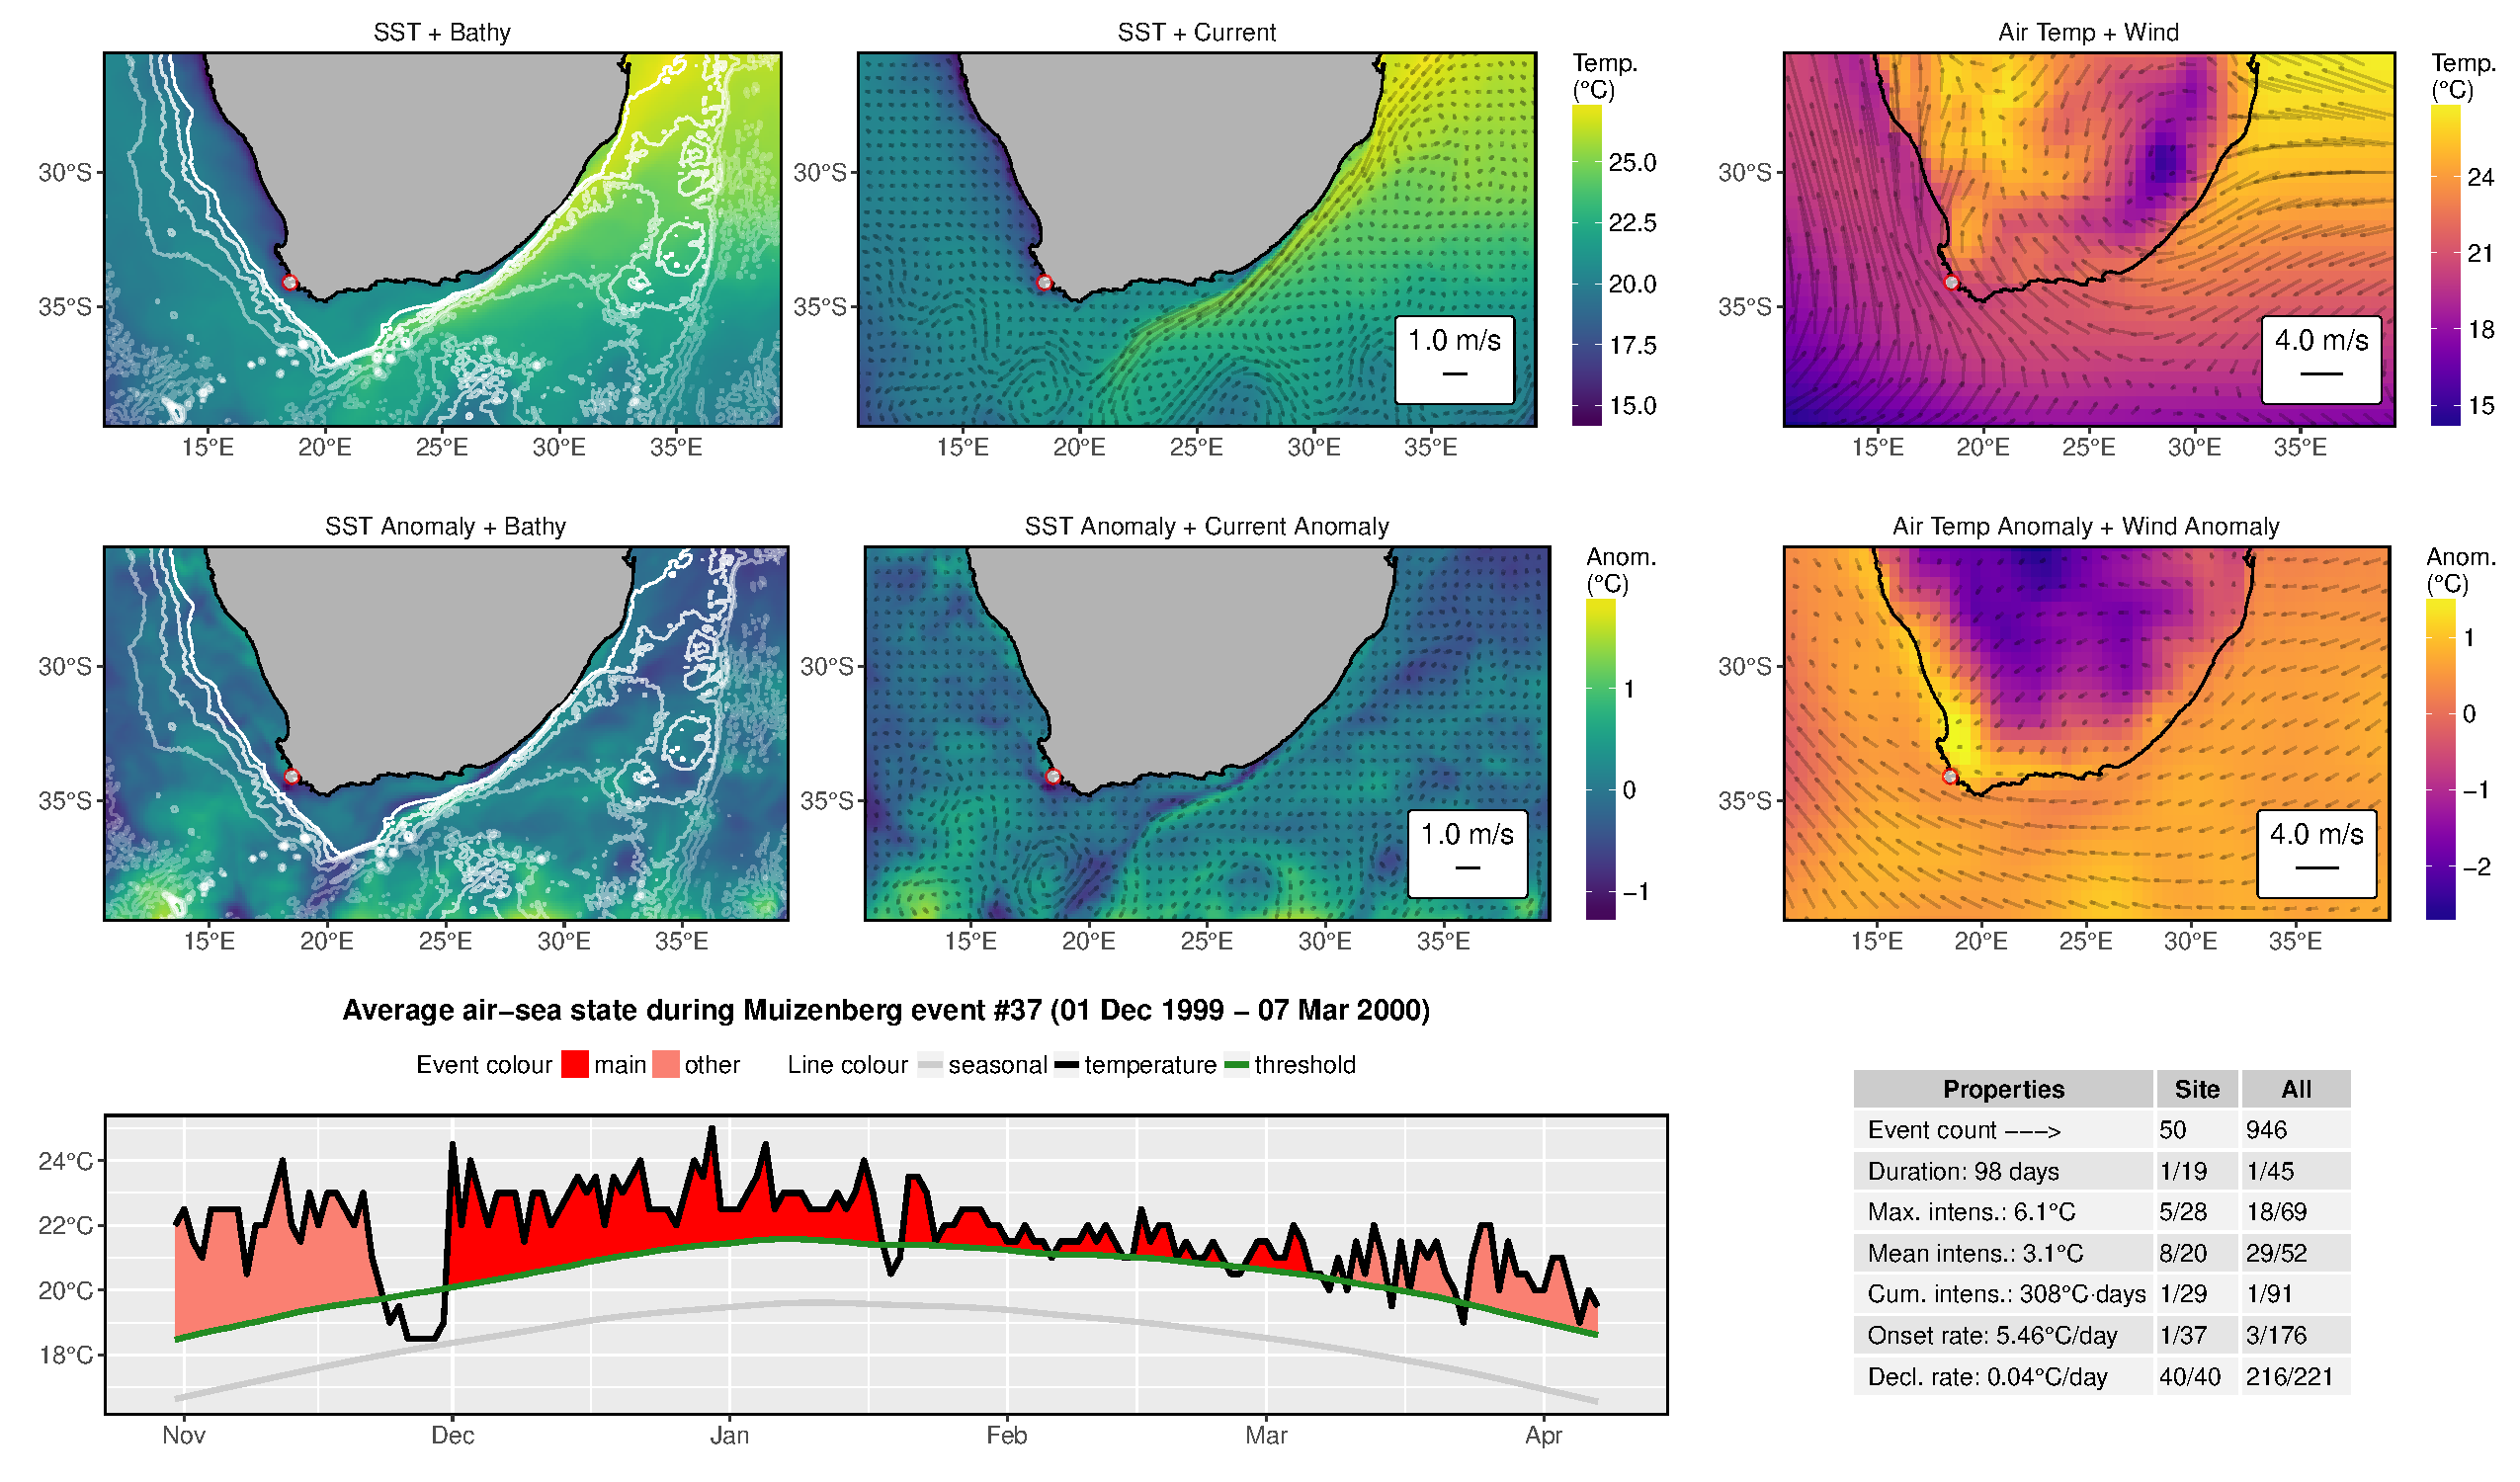
\includegraphics[width=1.0\textwidth]{figure_2.pdf}
\caption{An atlas figure for a single coastal marine heatwave (MHW). The location of collection for the \emph{in situ} coastal seawater temperature time series is shown in each of the top six panels as a white dot with a red border. The top row of panels shows the mean synoptic air and sea states during the MHW, created by averaging all daily synoptic air-sea states during the event. The middle row shows anomalies for the mean air and sea states during the event. The left hand panel in the bottom row shows the period of the time series in which the MHW occurred. The table in the bottom right corner shows the values for the relevant metrics of the event as explained in \Cref{table1} as well as its ranking against other events at the same site and the entire study area. Similar figures for each of the 86 MHWs used in this study are available here: https://github.com/schrob040/AHW/tree/master/graph/synoptic.}
\label{figure2}
\end{figure}

\subsection{Nonmetric multidimensional scaling (NMDS)}
% \subsection{Distinction between states}
With the calculation of the 366 daily climatologies for the air-sea states it was possible to determine if the air-sea states during the days in which a MHW was occurring (hereafter MHW states) differed from the average climatology air-sea states (hereafter climatology states). However, as the MHW state anomalies were to be used for all further analyses, it was necessary to also create climatology state anomalies against which to compare them. These climatology state anomalies were created by subtracting the average of all of the climatology states from each individual daily climatology. In order to reduce the dimensionality of the air-sea states down to a two-dimensional field to determine the potential relationship between the 86 MHW state anomalies and the 366 climatology state anomalies, nonmetric multidimensional scaling (NMDS) was used. NMDS was chosen as it is one of the most robust unconstrained ordination methods available \citep{Minchin1987}. Whereas the use of this technique is not wide-spread in climate science, we found that it was effective for reducing the dimensionality of the synoptic air-sea states used here. The temperature, U and V variables that make up each synoptic state, for all MHW and climatology states, were first scaled to a mean of zero within the variance of each variable. These scaled values were then converted into a Euclidean distance matrix before being fed into the NMDS algorithm. An additional benefit of NMDS is that it allows for the strength of the influence of the categorical variables within the data to be displayed on the resultant bi-plot as vectors, where the length of each vector represents the amount of influence that categorical variable has, and the direction of the vector shows where on the two-dimensional plain the ordinated data points are being influenced towards. The categorical variables considered when ordinating the MHW and climatology states together were the season during which the day or event occurred/started, as well as if the value represented a MHW or a climatology.

The goal of using NMDS to ordinate the states in this way is not to perform a statistical analysis on the data, indeed no significance is tested, but to visualise how each state relates to every other state while simultaneously visualising the effects of the categorical variables on the data. The resultant bi-plot generated by NMDS allows one to visually inspect the relationship between MHW and climatology states, in order to determine if they share a common pattern, or are indeed dissimilar from one another.

\subsection{Self-organising maps (SOMs)}
Several methods of clustering synoptic data have been employed in climate science. Of these K-means clustering is perhaps most often employed \citep[e.g.][]{Corte-Real1998, Burrough2001, Kumar2011}, with hierarchical cluster analysis (HCA) less so \citep[e.g.][]{Unal2003}. A newer technique, self-organizing maps (SOMs), has been gaining in popularity in climate studies \citep[e.g.][]{Cavazos2000, Hewitson2002, Morioka2010}. Here we have used a SOM to cluster the 86 MHW state anomalies.

The initialisation of a SOM is similar to more traditional clustering techniques \citep[e.g.][]{Jain2010} in that a given number of clusters (hereafter referred to as nodes) are declared by the user in order to instruct the SOM algorithm into how many nodes it should first randomly assign all of the data point \citep{Hewitson2002}. Each data point in this instance represents the anomalous air-sea state during a MHW and consists of temperature, U and V anomalies, which reach a total 9774 variables each. Therefore, each SOM node is represented not by a single value, but by a 9774 value long reference vector. After all of the data points have been clustered into a node, the SOM then determines the most suitable reference vector for each node to represent the data therein \citep{Hewitson2002}. The data points are then reintroduced to the SOM and, based on Euclidean distance, each data point is then matched to the node of 'best fit' \citep{Hewitson2002}. During this process the reference vectors for each node are modified as the SOM algorithm 'learns' how best to refine them to fit the data points, while also learning how best to fit the nodes in relation to one another \citep{Hewitson2002}. This means that not only does the SOM algorithm update the goodness of fit for each node during each run of the data, it also better orients the nodes against one another and allows better clustering of higher densities of similar data points (MHW state anomaly) \citep{Hewitson2002}. This allows the user to see not only into which node a given data point (MHW state anomaly) best belongs in, but also what the relationship between the nodes may be and how prevalent certain MHW state anomalies are over others. Here we initially allowed the SOM algorithm to iterate this process 100 times. Analysis of the resultant SOM showed that little progress was made in the fitting of the data after 40 iterations, and so 100 iterations was deemed appropriate.

Because the SOM algorithm was not able to provide consistent results each time the analysis was run on these data, we opted out of using the default random initialization (RI) method for the SOM in favour of principal component initialization (PCI). PCI differs from RI in that it uses the two principal components of the dataset, as determined from a principal component analysis (PCA) to initialize the choice of node centres for the SOM \citep{Akinduko2016}. This allows the SOM model to recreate the same results when it is run on the same data.

The appropriate number of nodes to use in a cluster analysis is an important decision \citep{Gibson2016a}. This is because it is necessary to include enough nodes to view a broad range of synoptic states, but not so many that the differences between the nodes become meaningless. Calculating the within group sum of squares (WGSS) as more nodes were included showed that 4 could be satisfactory, but that at least 6 would be better. Ultimately we settled on 9 nodes as this allowed for a wider variety of different synoptic air-sea states to be separated out from one another, allowing for a better understanding of the dominant patterns that exist during coastal MHWs. As proposed in \citet{Johnson2013}, the nodes that are output by a SOM should be significantly different from one another to ensure that an excess of nodes has not been used. Using an analysis of similarity we found this to be true for the choice of nine nodes (\emph{p} = 0.001).

Once each MHW state anomaly was clustered into a node a further mean air-sea state anomaly for each node was calculated by taking the average of all of the MHW state anomalies clustered within each node. It was these final mean air-sea state anomalies that were taken as the nine predominant air-sea patterns during coastal MHWs.

\section{Results}
\subsection{MHW states vs. Normal States}
When we plot MHW and climatology states on the same two axes of ordination within a bi-plot, we see in \Cref{figure3} that the climatology states are all clustered in an ellipsoid shape in the centre of the plot, whereas the MHW states are scattered along the top and bottom thirds. Furthermore, the seasons during which the climatology states occurred are clearly important to their ordination, whereas no clear pattern exists for the seasons of the MHW states. The vectors in \Cref{figure3} show in what direction the categorical variables in the dataset are influencing the placement of each data point (air-sea state) in the two-dimensional space. The four vectors for the four seasons each point towards the portion of the ellipsoid of climatology states of the corresponding season, and  the vector showing the direction towards which climatology (clim) states are shifted is nearly in the centre of the figure. The vector for the MHW states most closely resemble the vector for the autumn states.

\begin{figure}
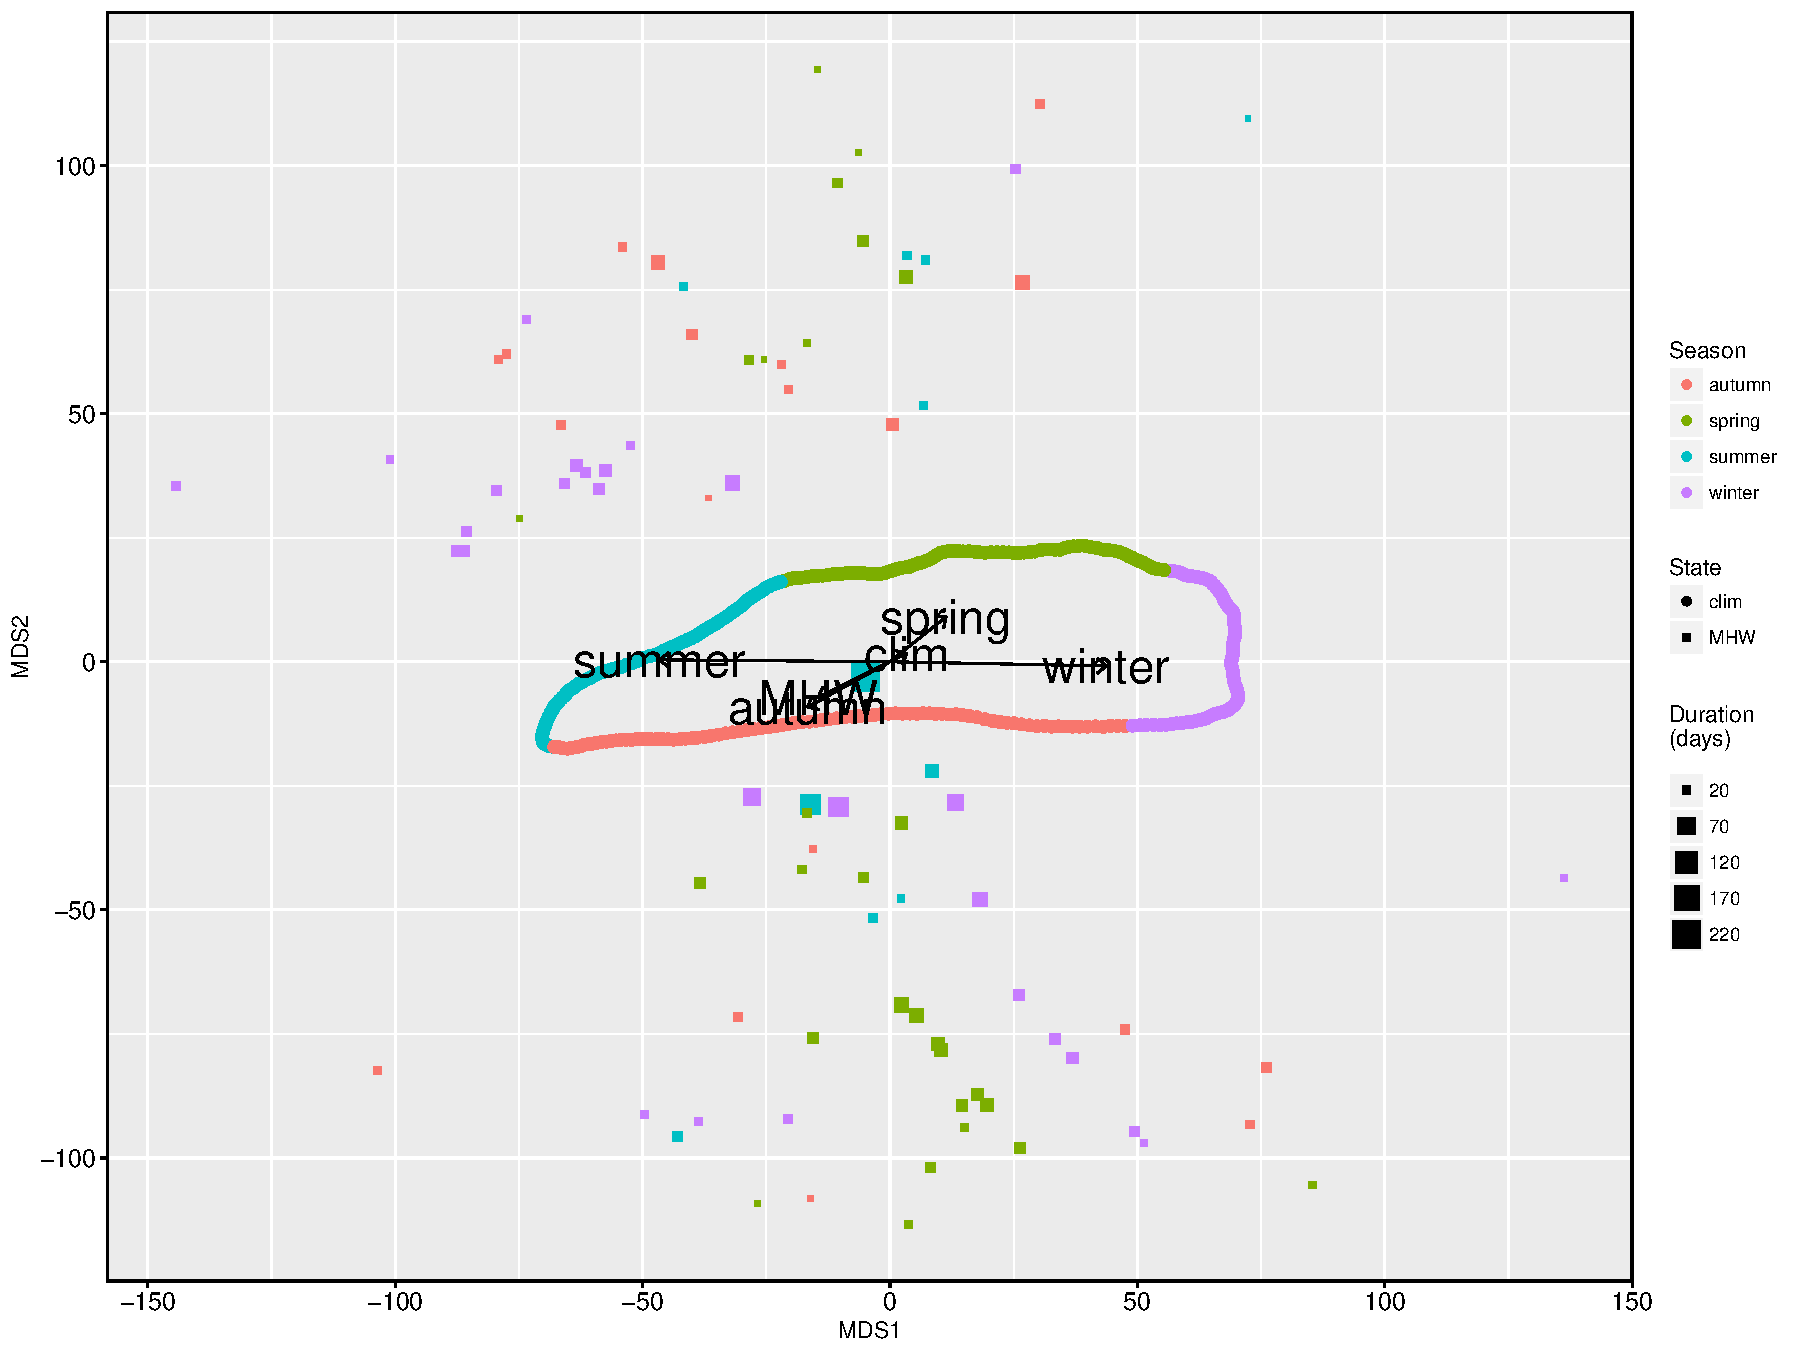
\includegraphics[width=1.0\textwidth]{figure_3.pdf}
\caption{Bi-plot showing the ordination of climatology (clim) states (circles) and marine heatwave (MHW) states (squares). The season of the year during which the state occurred/started is shown in colour. The influence of these two categorical variables, type of air-sea state and season of occurrence, on the placement of each state in a two-dimensional space are shown as black labelled vectors. Note that the clim states (circles) are plotted so tightly together that they do not appear as individual points.}
\label{figure3}
\end{figure}

\subsection{MHW patterns}
The nine predominant anomalous air-sea patterns around southern Africa during coastal MHWs may be seen in \Cref{figure4}. The SST anomalies generally increase as one moves towards the top left panels. The air temperature anomalies increase as one moves towards the right panels. The current anomalies are only slightly greater towards the top panels. The wind anomalies show the most clear gradient across the panels with strong north-westerly anomalies in the top left corner giving way to strong easterly anomalies in the bottom right panels. The air and sea patterns apparent in each individual node are described below.

\begin{figure}
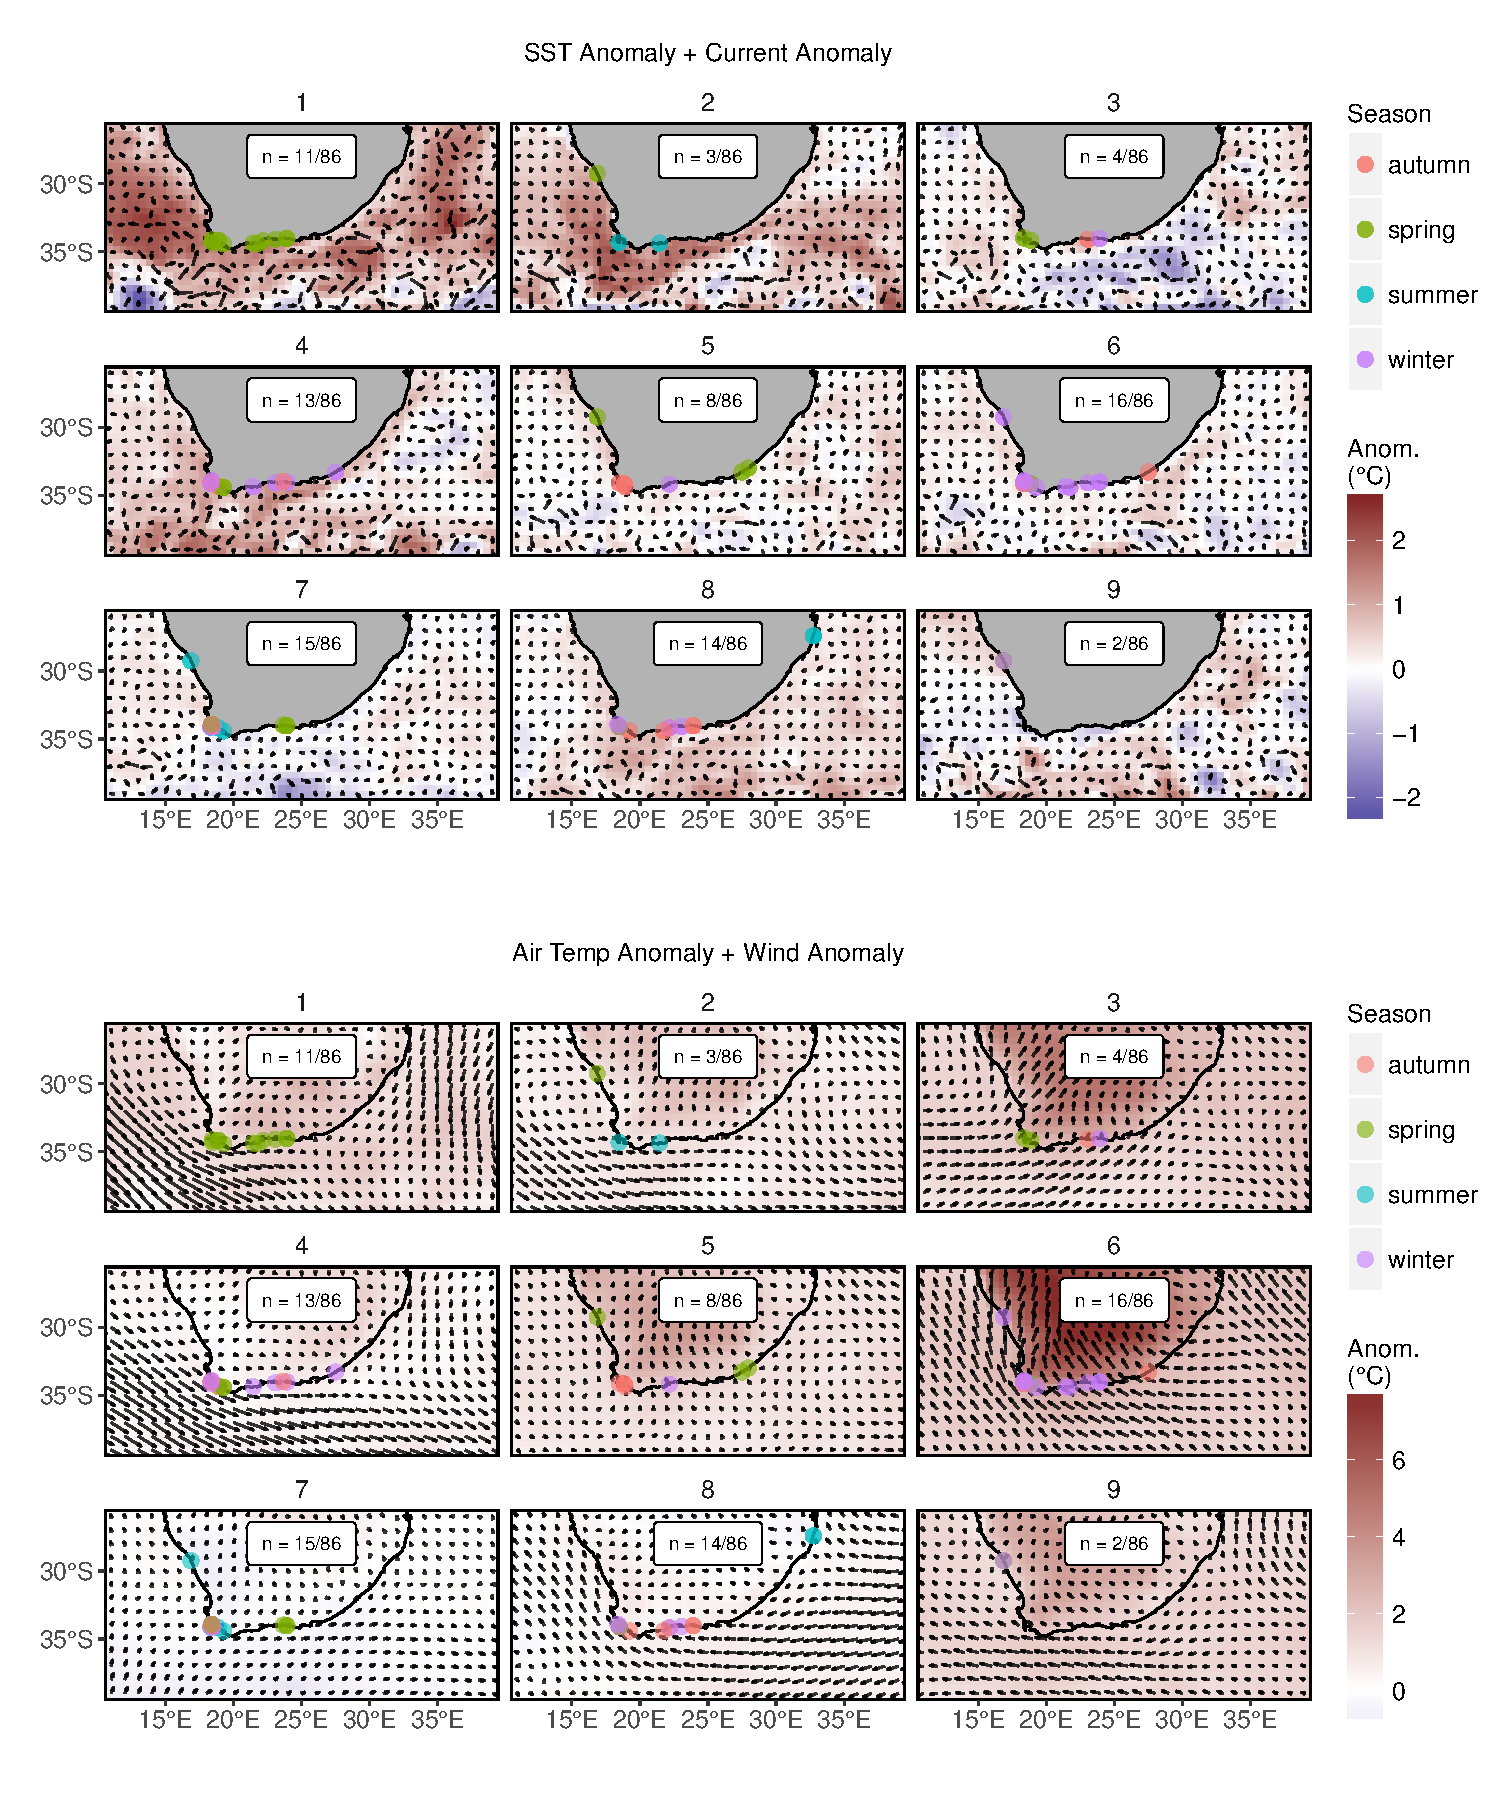
\includegraphics[width=1.0\textwidth]{figure_4.pdf}
\caption{Predominant anomalous air and sea patterns during coastal marine heatwaves (MHWs) as determined by a SOM. The top nine panels show the sea patterns while the bottom nine panels show the air patterns. The current and wind vectors are the same scale as those found in the respective air and sea panels of \Cref{figure1}. The number of events clustered into each node is shown within the white label in the middle of each panel. The location of each coastal MHW within each node is shown with a dot whose colour denotes the season during which that event occurred/started. Note that the temperature anomaly scales differ for the top and bottom nine panels.}
\label{figure4}
\end{figure}

\subsubsection{Node 1}
Node 1 showed the most striking oceanic pattern out of all of the nodes (\Cref{figure4}). The mean sea pattern from all of the MHW states clustered into this panel showed  Agulhas Current leakage into the Atlantic as well as forcing onto the coastal region around the Cape Peninsula and potentially along the rest of the south coast. The SST anomaly along the coast, as well as in the open ocean was also the warmest of all of the panels. The air temperature anomaly was mild relative to the other nodes but very strong north westerly wind anomalies were present to the west of the subcontinent and strong northerly wind anomalies to the east. The wind anomalies from the north west moved south of the subcontinent and continued along the south coast up to the location of the occurrence of the most eastward MHW before encountering the Indian high and abating. Neither of the high pressure cells showed any real influence on the overland wind anomalies.

\subsubsection{Node 2}
Node 2 showed similar warm SST anomalies in the nearshore along the west and south coasts as Node 1, with open ocean anomalies being cooler. There appeared to be some onshore forcing and leakage of the Agulhas current but it was not as strong as in Node 1. The air temperature and wind anomalies in this panel were slightly less than Node 1 as well. The Indian and Atlantic highs appear shifted slightly more to the south west with the westerly wind anomalies along the bottom of the panel reaching further east. The anomalous offshore wind circulation did not appear to move onshore.

\subsubsection{Node 3}
Node 3 showed little in the way of strong positive SST anomalies, with much of the water south of the subcontinent having negative SST anomalies during the events clustered into this node. There were some atypical surface currents occurring to the south west of the Cape Peninsula, similar to nodes 1 and 2, and may signify the presence of Agulhas leakage. The overland air temperature anomalies were strong in this node with westerly wind anomalies pushing onshore along the west and south coasts from the south west and continuing overland. These onshore south westerlies were met on the eastern side of the subcontinent by weak Indian high anomalies.

\subsubsection{Node 4}
Node 4 showed Agulhas leakage and onshore forcing with warm coastal SST anomalies along all three coasts. Open ocean SST and current anomalies were relatively even, with a large stretch of anomalously warm SSTs and Agulhas retroflection along the bottom of the panel. Air temperature anomalies were relatively even, though slightly warmer over land than the sea. The wind anomalies were similar to nodes 1 and 2, but with the largest western wind anomaly component of all of the nodes.

\subsubsection{Node 5}
Node 5 showed some atypical currents to the south west of the Cape Peninsula, similar to most of the nodes. The SST anomalies during the events in this node were a mix of warm and cold, with mild warm anomalies present along most of the coast. The air temperature anomalies, particularly overland, were strong during these events. Even though the wind anomalies were slight over the ocean during the events in this node, they were stronger overland were anomalous onshore wind movement occurred.

\subsubsection{Node 6}
The surface current and SST anomalies in node 6 were very similar to node 5, with fewer warm SST anomalies along the coast. The air temperature anomalies overland during these events were in excess of 7\degree C with strong south easterly wind anomalies pushing not only onshore, but along the entire study area as well. The events clustered into this node had the greatest air temperature anomalies of all the nodes.

\subsubsection{Node 7}
Node 7 showed some atypical currents to the south west of the subcontinent but little in the way of onshore forcing or warm SST anomalies. The Southern Ocean appeared to be pushing up into the study area during these events as seen by the cold anomaly in the bottom middle of the panel. The air temperatures showed a very slight negative anomaly over much of the study area with very weak westerlies winds along the southern portion of the study area.

\subsubsection{Node 8}
Node 8 showed warm SST anomalies for all but the offshore portion of the Atlantic Ocean. There was some atypical vorticity along the south of the study area, but this was moving away from the coast and there appeared to be little leakage of the Agulhas current. The air temperature anomalies during these events were small with strong easterly wind anomalies moving across the entire study area. These wind anomalies wrapped around the subcontinent, rather than moving onshore.

\subsubsection{Node 9}
The final node showed cold SST anomalies along much of the south coast, with some warm anomalies further south and atypical vorticity to the south east that did not appear to be reaching the coast, but could represent Agulhas leakage. The wind during the events in this node was anomalously strong from the east with warm air temperature anomalies over the land and sea. There is some onshore movement of wind anomalies along the entire coastline.

\subsection{Temporal patterns}
MHWs that occurred during summer were only present in nodes 2, 7, \& 8 (\Cref{figure5}) and were the least common, with winter and spring events occurring more than twice as frequently (\Cref{table2}). Clustering of autumn, winter, and spring events that occurred over a range of years may be found in 6 of the 9 nodes. The most notable exception to what is otherwise a lack of a clear temporal pattern in the clustering of the MHW states is node 1. All of the MHWs in node 1 occurred during the spring of 2004 within days of one another. Of the 13 events clustered into node 4, 11 of them occurred during the same year, though over a span of several months. Node 6 also shows a strong affinity for events from only one season with 13 of the 16 MHW therein having occurred during winter, but were spread out from 1993 to 2014. The clustering of events that occurred concurrently is consistent throughout these results with the exception of node 9. More than half of the summer events were clustered into node 7, and nearly half of all winter events were clustered into node 6. The highest concentration of spring events may be found in node 1 however, every node contains at least one spring event. Autumn events were absent in 3 nodes, but were otherwise the most evenly distributed.

\begin{figure}
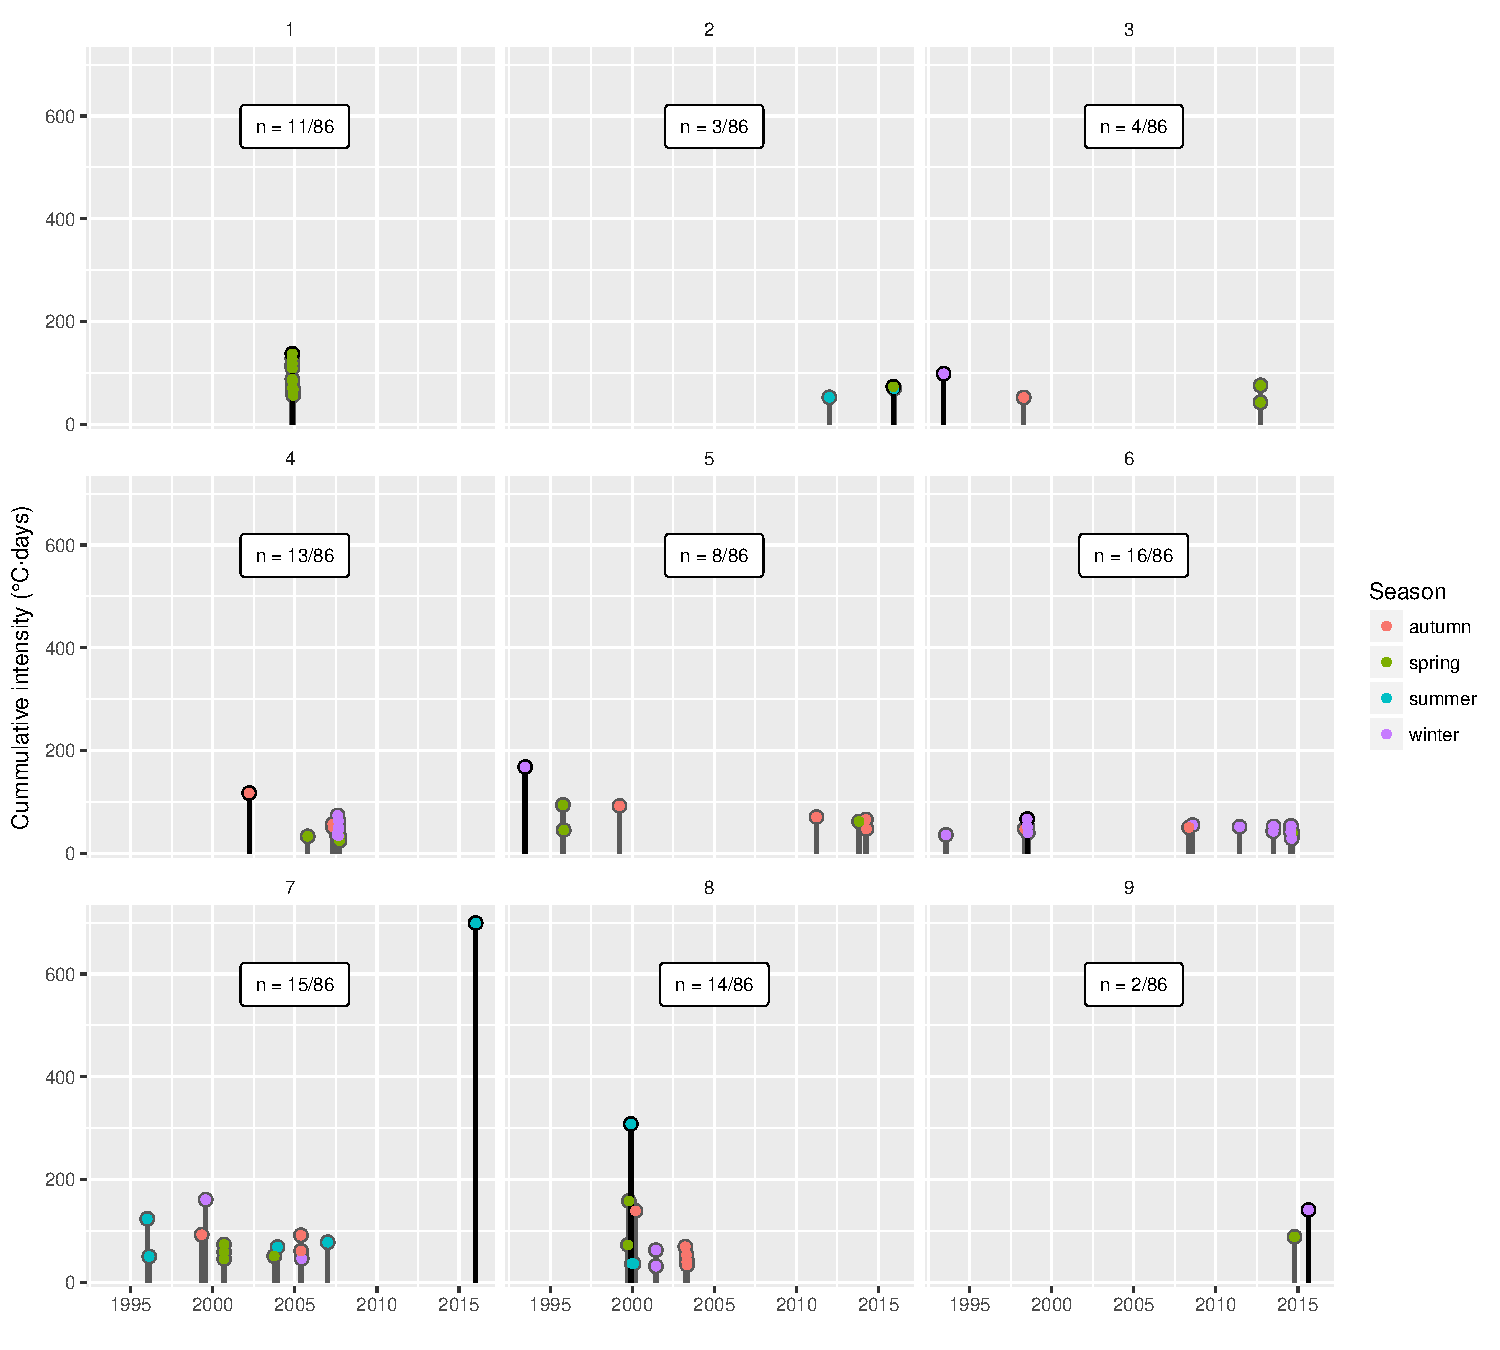
\includegraphics[width=1.0\textwidth]{figure_5.pdf}
\caption{Lolliplot showing the start date for each marine heatwave (MHW) within each node as seen in \Cref{figure4}, with the number portion of total events per node shown within the white label in the middle of each panel. The height of each lolli shows the cumulative intensity of the event, as outlined in \Cref{table1}, while the lolli colour denotes the season during which the event occurred/started.}
\label{figure5}
\end{figure}

\begin{table}[ht]
\caption{\small The count, seasons, and relevant metrics for the MHWs found within each node. The mean duration of the events within each node is shown in the \emph{D} column with the \emph{i\textsubscript{cum}} and \emph{i\textsubscript{max}} columns showing the mean cumulative and maximum intensities respectively (\Cref{table1}). The bottom row of each column shows the sum or mean of the column as appropriate.}
\label{table2}
\centering
\tiny
\begin{tabular}{cccccccccccc}
  \toprule
node & count & summer & autumn & winter & spring & west & south & east & \emph{D} & \emph{i\textsubscript{cum}} & \emph{i\textsubscript{max}} \\
  \midrule
  1 &  11 &   0 &   0 &   0 &  11 &   0 &  11 &   0 & 33.50 & 93.73 & 4.04 \\
  2 &   3 &   2 &   0 &   0 &   1 &   1 &   2 &   0 & 21.30 & 64.88 & 4.05 \\
  3 &   4 &   0 &   1 &   1 &   2 &   1 &   3 &   0 & 25.80 & 67.19 & 3.49 \\
  4 &  13 &   0 &   3 &   7 &   3 &   4 &   9 &   0 & 25.20 & 51.07 & 2.89 \\
  5 &   8 &   0 &   4 &   1 &   3 &   1 &   6 &   1 & 29.00 & 80.52 & 4.75 \\
  6 &  16 &   0 &   2 &  13 &   1 &   5 &  11 &   0 & 23.40 & 47.59 & 2.94 \\
  7 &  15 &   6 &   3 &   2 &   4 &   8 &   7 &   0 & 41.10 & 118.55 & 4.21 \\
  8 &  14 &   3 &   6 &   3 &   2 &   1 &  11 &   2 & 28.20 & 79.50 & 3.94 \\
  9 &   2 &   0 &   0 &   1 &   1 &   2 &   0 &   0 & 46.00 & 114.56 & 4.78 \\
  ALL &  86 &  11 &  19 &  28 &  28 &  23 &  60 &   3 & 29.90 & 77.72 & 3.73 \\
  \bottomrule
  \end{tabular}
\end{table}

\subsection{Spatial patterns}
\Cref{figure4} shows that, with the exception of Node 9, the SOM clustered MHWs together that were separated over large distances and by oceanographically dissimilar features. Only Nodes 1 and 9 contained events that occurred on only one of the coasts. Additionally, only 3 of the 86 MHWs in this study occurred on the east coast and these events were found within Nodes 5 and 8, which contain events from all three coasts.

\subsection{MHW metrics}
\Cref{table2} shows that largest values for duration (\emph{D}), cumulative intensity (\emph{i\textsubscript{cum}}) and maximum intensity (\emph{i\textsubscript{max}}) were more than twice that of the smallest values. Nodes 7 and 9 show the longest mean durations however, with Nodes 2 and 6 the shortest. As large cumulative intensities are generally a product of lengthy MHWs, it is not surprising to see that nodes 7 and 9 also have the highest values for this metric. Nodes 6 and 4 have the lowest cumulative intensities. Maximum intensity is not a function of duration however, we still see that node 9 has the greatest value. Node 5 is a close second. Node 9 may have the greatest values for all 3 metrics however, it only contains two events, making node 7, which has the second overall largest events, a better representation of the air-sea states during very large events. Nodes 6 and 4, as seen in \Cref{figure4}, are good representations of air-sea states during the smaller events used in this study.

\section{Discussion}
\subsection{MHW states vs. Climatology States}
As one may see from the flat ellipse of multi-coloured circles in \Cref{figure3} (the climatology states), the variance represented along the x axis of the bi-plot is seasonality. The MHW states (squares) are spread out more along the y axis. This then must be aseasonal variance, likely the anomalous characteristics of air and or sea that occur during the events. This shows that these aseasonal characteristics are largely independent from the daily climatologies during any given time of the year. The MHW states are distributed either above the summer/spring portion of the climatology state ellipse, or below the autumn portion of the ellipse, and not near the winter portion. The closer to the climatology ellipse a MHW state is, the more it resembles the seasonal climatology that occurs during that portion of the ellipse. Very few MHW states were near climatology states of the same season (e.g. winter MHW states may generally be found above the summer climatologies or below the autumn climatologies), and only one MHW state is remotely close to the winter portion of the ellipse. This means that in addition to being set apart from the climatology states by aseasonal variance, the seasonal signal present in the MHW events almost always represents a different season than the one in which the event occurred. Furthermore, all but one of the MHW states showed a seasonal signal that was different from anything that occurred during the winter climatologies. This is not surprising, as one would assume that MHWs would occur during warm air or sea states, and winter is the coldest time of the year. More interesting was that the majority of MHW states most closely resembled the climatology states during autumn, with spring and then summer as second and third. An initial assumption with MHWs states could be that they should most closely resemble the warmest time of year, summer. That they are instead ordinated more closely with autumn and spring climatologies means that there is something peculiar about the times of transition across the seasons. During summer and winter months in southern Africa the Atlantic and Indian highs tend to stay in place latitudinally \citep{vanHeerden1998}. It is during autumn and spring that, not always in a predictable manner, the synoptic atmospheric features around the subcontinent migrate north or south \citep{vanHeerden1998}. As these systems shift they create patterns that appear most similar to the patterns that occur during the large coastal MHWs in this study.

\subsection{MHW patterns}
The most notable sea state pattern from the clustering of these events has been Agulhas leakage. This phenomenon is when warm Indian Ocean water bursts into the colder Atlantic Ocean \citep{Beal2011}. These warm eddies then typically spin up along the west coast. This transport of a large body of atypically warm water along a large stretch of coastline is a similar finding to the cause of the Western Australia MHW in 2011 where an unusual surge of the Leeuwin Current forced a large body of anomalously warm water onto the coast \citep{Feng2013, Benthuysen2014}. This onshore forcing of water is most apparent in node 1 (\Cref{figure4}) however, Nodes 2, 4, and (to a lesser extent) 3 show a similar though less pronounced oceanic pattern, meaning that roughly one third of the events in this study occurred during Agulhas leakage. These four Agulhas leakage-dominated nodes also share the same anomalously warm air temperatures and north westerly to westerly wind patterns, to varying degrees. Node 3 differs slightly from the other three Agulhas leakage-dominated nodes in that the SST anomalies are not large, but the air temperature anomalies are, with a warm air low pressure cell present over the subcontinent (lacking in the other 3 nodes), allowing onshore wind anomalies. Excluding node 3 from the patterns present during Agulhas leakage, we see that a common state is warm coastal SST anomalies occurring during Agulhas leakage while a strong north-westerly wind anomaly (strong Atlantic high) exists in contrast to weak south-easterly (weak Indian high) wind anomalies and concurrently with a westerly wind anomaly that may be drawing aseasonally close to the subcontinent. One of the primary causes of Agulhas leakage is when a weak Indian high does not provide enough of the positive wind stress curl the current needs to have enough inertia to retroflect against the Benguela current \citep{Beal2011}. The second feature that allows Agulhas leakage is when the latitude zero wind stress curl caused by the westerly wind belt has shifted further south of the subcontinent \citep{Beal2011}. We see in the Agulhas leakage panels that Indian high anomalies are much weaker than the Atlantic, allowing a loss in inertia of the Agulhas current and an increased risk of leakage however, the westerlies appear to be shifted further north, which should inhibit leakage. These two diametric forces contributing to the air-sea states during the Agulhas leakage may be what is causing the Agulhas to move so close to the shore, leading to the large SST anomalies seen there.

Node 8 also shows some onshore forcing of the Agulhas current, but with no large leakage into the Atlantic Ocean. Strong nearshore SST anomalies exist, but no ensuant leakage into the Atlantic due to the strong Indian high anomalies during the events in node 8 that likely increased the inertia of the Agulhas current enough that it retroflected against the Benguela current, while still forcing warm water onto the coast. Node 8 is also 1 of only two nodes that contain events from all three coasts, meaning that a strong Agulhas pushing onto the coast is a common pattern during MHW along the coastline of the entire study area.

Taken together with the events that occurred during Agulhas leakage, over half of the MHWs in this study occurred during some sort of anomalous Agulhas behaviour coupled with warm nearshore SST anomalies. This is strong support for the relationship between the Agulhas current and coastal MHWs. \citet{Beal2011} state, while difficult to say with certainty, Agulhas leakage is likely to increase under the continued regime of global anthropogenic warming. This then implies that large MHWs like those seen in nodes 1, 2, 3, 4 and 8 are likely to increase.

With the exception of nodes 7 and 8, all of the atmospheric states during coastal MHWs showed warm air temperature anomalies. The largest of these anomalies occurred in node 6 (mostly winter events), with overland temperature anomalies in excess of 7\degree C. It is also worth noting that the anomalies overland are generally greater than over the sea, and that the wind anomaly patterns during coastal MHWs ranged from a strong Atlantic high to a strong Indian high. From this one must infer that air temperatures will almost always be anomalously warm during a coastal MHW and that winds will usually either be anomalously strong from the north-west or south-east. Furthermore, the nodes with the greatest overland air temperature anomalies (3, 5, 6, and 9) had comparable amounts of cold and warm SST anomalies as well as onshore wind anomalies. This implies that the MHWs in these nodes were forced by the onshore winds occurring during warm atmospheric anomalies and not by oceanic conditions. This could have caused MHWs in one of two ways. The first would be through direct atmospheric heating of the shallow nearshore water, as occurred over the Mediterranean in 2003 \citep{Garrabou2009}. The second being that the anomalous onshore wind movement could have prevented seasonally regular wind forced upwelling from occurring, which would have then caused the coastal water at the location of the event to appear aseasonally warm. Taken together the events in these nodes account for roughly one third of the events in this study.

The lack of a strong air or sea pattern in node 7 implies that the 15 events that were clustered there do not share any common pattern. Meaning that there may still be many MHWs that occur not because of any recurrent or predominant air or sea pattern. This is an important finding as it shows that even though clear patterns in air and sea may exist during most MHWs, these events may still occur during entirely novel conditions. A different interpretation of the lack of an apparent pattern in node 7 is that because the events clustered into that event were the longest, on average, of all of the events in this study, creating a mean air-sea state for the entire duration of each event was impractical. That enough variation in air and sea would have occurred over the lifespan of the event so as to 'smooth out' any apparent signal. If this is so, it does serve to address what may have caused such a large event. The atlas figures for each event in node 7, (https://github.com/schrob040/AHW/tree/master/graph/synoptic), show that there are indeed patterns in the air-sea anomalies during these events, and that they do differ from the patterns in the other nodes.

A final note on the patterns visible in \Cref{figure4}. The south west corners of the sea states in Nodes 2, 3, 5, 6, 7, and 9, show an almost identical anticyclonic (clockwise) anomaly on the exact same pixels. Upon more minute investigation it was determined that this anticyclone, likely an Agulhas ring \citep{Hutchings2009}, occurred between roughly 12.5\degree E to 14.5\degree E and 35.5\degree S to 37.5\degree S. This eddy occurred during exactly two thirds of all of the events in this study, making it the most common air or sea pattern found.

\subsection{Temporal patterns}
With the exception of node 1, the nodes produced by the SOM contain events not only over several years, but during two or more seasons as well. This means that the typical patterns that occur during MHWs are not bound to any particular season, and may occur during any time of the year. An exception to this finding is that even though node 6 did contain purely winter events, 13 of the 16 events clustered into that node were, and this is strong support for the predictive potential of a strong overland air temperature anomaly during winter months being linked to coastal MHWs.

We found, to some surprise, that only a small portion (\Cref{table2}) of MHWs occurred during summer months. This implies that the phenomenon that may be driving the long MHWs in this study occur more often during the cooler months of the year. This may mean that summer months around southern Africa are more stable than at other times of the year, or again that the processes that drive long MHWs are linked to the transitioning of warmer temperatures to cooler temperatures and \emph{vice versa}.

\subsection{Spatial patterns}
That 7 of the 9 nodes created by the SOM consist of synoptic air-sea states that occurred during MHWs on different coastal sections of the study area, separated by thousands of kilometres of coastline and distinct oceanographic and atmospheric boundaries, was somewhat surprising as more distinct clustering of events from different coasts was anticipated. That almost all nodes contain synoptic or meso-scale air-sea patterns that may cause MHWs on the west or south coast implies that the forces that cause MHWs are large, and able to exist simultaneously across typical air and sea barriers.
% The first being that onshore forcing of the Agulhas current during the MHWs on the south coast may be crreping past the Benguela current along the coast, even when Agulhas does not appear to be present. The second being that the MHWs may be forced by temperature exchange between air and sea at the coast. With the third likely candidate being onshore forcing of wind preventing seasonally consistent upwelling.

Of the 86 MHWs included in this study, only 3 occurred on the east coast. This means that the east coast is much more thermally stable than the other two coasts however, it is also difficult to determine any potential relationships between synoptic patterns that may be responsible for events only on the east coast, or between the east coast and the south or west coasts.

\subsection{MHW metrics}
The most seasonally predictable MHWs, those occurring during winter months and clustered into node 6, where also the shortest and weakest (\Cref{table2}). As these events were clearly a product of thermal heating (\Cref{figure4}), one could infer that atmospheric forcing of MHWs causes less dramatic events than those forced by the ocean. This would be an incorrect inference to draw as the MHWs clustered in node 5, which also contain a clear atmospheric signal, have a greater cumulative intensity than most of the Agulhas leakage nodes. The largest events, those in node 7, contain such disparate air-sea states that the mean air and sea patterns seen in \Cref{figure4} appear to be almost blank. These factors prevents a conclusion to be drawn on whether the sea or air may cause the largest MHWs.

\section{Conclusion}
This research has highlighted that coastal MHWs with durations in the 10th percentile of all MHWs detected along the coast since 1993 often occur during the abnormal advection of warm water onto the coast due to atypical Agulhas Current activity, or when warm air centred over land coincided with strong onshore winds. Along the west and south coasts of southern Africa the offshore water is often warmer than coastal waters and so even if the offshore waters are not aseasonally warm at their point of origin, they may still cause a coastal MHW. Anomalous wind and air temperature patterns during coastal MHWs were found to cover a wide range of states from strong Atlantic highs with weak Indian highs to weak Atlantic highs with strong Indian Highs. Anomalous movement of winds onshore during high overland temperatures and low pressure cells were also a common pattern. The most consistent pattern found to occur most consistently during MHWs was a sub-meso-scale anticyclonic eddy, roughly 2 degrees wide and centred at 13.5\degree E and 36.5\degree S, but we did not investigate the ocean dynamics implied by the presence of this eddy as that was beyond the scope of this study.

We found that the air-sea states during coastal MHWs did not relate closely to the daily climatology air-sea states seen throughout the year. This means that the patterns that occur during these MHWs are not represented by typical seasonal conditions. Furthermore, the fewest MHWs occurred during summer months than any other season. These two facts taken together support the argument that MHWs are not simply a symptom of solar heating during the warm months of the year, but that other aseasonal phenomena are having a more pronounced effect on the atypical warming we have documented. It is also possible that large MHWs are recorded less frequently during summer months because coastal waters will be warmer, and incursions of offshore water, or atmospheric heating will not cause a large enough difference in the expected daily temperature to be flagged as a MHW.

The mean air-sea state during the longest, most cumulatively intense events also had the smallest temperature and current/wind anomalies, meaning that for the majority of the MHWs included in this study that have the greatest potential to cause the most negative impact on nearshore ecosystems, there does not appear to be a consistent air or sea pattern. Rather, most of the largest events occurred during a somewhat novel air-sea pattern that was not repeated often enough over time to be clustered into their own node.

The methodology utilised here has shown that it is possible to discern predominant air and sea patterns that occur during MHWs; however, one must have knowledge of the synoptic and meso-scale oceanic and atmospheric properties of the study area in order to correctly interrogate those results. Even with this knowledge, many of the largest MHWs did not show any relationship to these potential synoptic or meso-scale forces. One must therefore not assume that such broad patterns in either the air or sea may be at the root of any single MHW observed in nearshore environments. Finer spatial resolutions should also be considered when investigating individual events. This is however challenging as such high resolution \emph{in situ} data are often very sparse. It is therefore advised that areas of particular susceptibility to MHWs be identified in order to allow for finer scale monitoring of these areas to be supported. Once these areas have been identified and such monitoring systems installed, it may then be possible to better determine what leads to coastal MHWs.

The findings here that certain patterns do exist during MHWs is a strong first step to developing a system of prediction for these potentially dangerous events. The ERA-Interim dataset lends itself well to this regard. Unfortunately there are currently no reanalysis products available that accurately forecast the complex Agulhas Current \citep{Cooper2014} and so this presently inhibits the development of a predictive system based on air-sea forecasting.

In order to determine potential patterns that may or may not exist during MHWs, this study utilised air and sea surface temperatures and velocity vectors. This was done because of the few large MHWs whose causes were known, \citep[e.g.][]{Garrabou2009, Feng2013, Pearce2013, Benthuysen2014, Chen2015a, Oliver2017} most were best related to these variables. Having shown that temperature and surface vorticity patterns do exist during coastal MHWs, a follow up to this study should analyse surface pressure, which was the main driver of the ``The Blob'' \citep{Bond2015a}, as well as eddy kinetic energy (EKE), which was a primary driver of the 2015/16 Tasman Sea MHW \citep{Oliver2017}.

\section*{Acknowledgements}
We would like to thank DAFF, DEA, EKZNW, KZNSB, SAWS and SAEON for contributing all of the raw data used in this study. Without it, this article and the South African Coastal Temperature Network (SACTN) would not be possible. This research was supported by NRF Grant (CPRR14072378735). This paper makes a contribution to the objectives of the Australian Research Council Centre of Excellence for Climate System Science (ARCCSS). The authors report no financial conflicts of interests. The data and analyses used in this paper may be downloaded at https://github.com/schrob040/MHW. The metadata for each SACTN time series used in this study may be downloaded at https://github.com/schrob040/AHW/blob/master/setupParams/SACTN\_site\_list.csv.

\section*{References}

% Eric's paper outlining the methodology
% Oliver, E. C. J., V. Lago, N. J. Holbrook, S. D. Ling, C. N. Mundy, A. J. Hobday (2017), Eastern Tasmania Marine Heatwave Atlas, Institute for Marine and Antarctic Studies, University of Tasmania. doi: 10.4226/77/587e97d9b2bf9. http://metadata.imas.utas.edu.au/geonetwork/srv/eng/metadata.show?uuid=20188863-0af6-4032-98f8-def671cdaa58

% Citing ERA-interim
% http://onlinelibrary.wiley.com/doi/10.1002/qj.828/abstract

% Disable the following line when wanting to repopulate the .bbl file from the AHW.bib file
%\bibpunct{(}{)}{;}{a}{}{,} % Not certain this line is necessary...

\bibliography{AHW} % Comment out when manually copying the references from the .bbl file
% Delete all of the following when using the AHW.bib file with the above line
% No one here but us chickens...
% Delete the above line when using the AHW.bib file instead of copying in the .bbl file

\end{document}